%%%%%%%%%%%%%%%%%%%%%%%%%%%%%%%%%%%%%%%%%%%%%%%%%%%%%%%%%%%%%%%%%%%%%%
% Based on LaTeX Template: Newsletter  
% Source: http://www.howtotex.com
%
% Adapted for Nebraska Ornithologists' Union Burrowing Owl
% 
%%%%%%%%%%%%%%%%%%%%%%%%%%%%%%%%%%%%%%%%%%%%%%%%%%%%%%%%%%%%%%%%%%%%

% important things to run first

% use lualatex

%!TEX program = lualatex

%% Tag PDF for accessibility

\DocumentMetadata{
	lang        = en,
	pdfstandard = ua-2,
	pdfstandard = a-4f, %or a-4
	tagging     = on
} 

\documentclass[10pt,letterpaper]{article}

%%% ---------------
%%% PREAMBLE
%%% ---------------


% Define geometry (without using the geometry package)
\setlength\topmargin{-48pt}
\setlength\headheight{0pt}
\setlength\headsep{25pt}
\setlength\marginparwidth{-20pt}
\setlength\textwidth{7.0in}
\setlength\textheight{9.5in}
\setlength\oddsidemargin{-30pt}
\setlength\evensidemargin{-30pt}

% remove double spacing after periods
\frenchspacing

\usepackage[english]{babel}			% english
\usepackage{graphicx}				% images
\usepackage{amssymb,amsmath}		% math
\usepackage{multicol}				% three-column layout
\usepackage{url}				% URL package
\usepackage{marvosym}				% symbols
\usepackage{wrapfig}				% wrapping text around figures
\usepackage[T1]{fontenc}			% font encoding
\usepackage{charter} 				% Charter font for main content
\usepackage{blindtext}				% dummy text
\usepackage{datetime}				% custom date
\newdateformat{mydate}{\monthname[\THEMONTH] \THEYEAR}

\usepackage[pdfpagemode=FullScreen,
			colorlinks=true,
			linkcolor=blue]{hyperref}	% links and pdf behaviour

% Customize (header and) footer
\usepackage{fancyhdr}
\pagestyle{fancy}
\lfoot{	\footnotesize 
		Burrowing Owl \\
		\Mundus\ \href{https://noubirds.org/}{NOUbirds.org}	\quad
		% \Telefon\ 555-5555											\quad
		%\Letter\ \href{mailto:frits@howtotex.com}{frits@howtotex.com}
	  }
\cfoot{}
\rfoot{\footnotesize ~\\ Page \thepage}
\renewcommand{\headrulewidth}{0.0pt}	% no bar on top of page
\renewcommand{\footrulewidth}{0.4pt}	% bar on bottom of page

%%% ---------------
%%% DEFINITIONS
%%% ---------------

% Define separators
\newcommand{\HorRule}[1]{\noindent\rule{\linewidth}{#1}} % Creating a horizontal rule
\newcommand{\SepRule}{\noindent							 % Creating a separator
						\begin{center}
							\rule{250pt}{1pt}
						\end{center}
						}						

% fonts
\usepackage{fontspec}
%\newfontfamily{\lexend}{Lexend}
% \DeclareTextFontCommand{\cwy}{\cherokeefam}

% Define Title en News input
\newcommand{\JournalName}[1]{%
		\begin{center}	
			\Huge \fontspec{QTBrushStroke}
			%\usefont{T1}{QTBrushStroke}{m}{n}
			#1%
		\end{center}	
		\par \normalsize \normalfont}
		
\newcommand{\JournalIssue}[1]{%
		\hfill \textsc{\mydate \today, No #1}
		\par \normalsize \normalfont}

\newcommand{\NewsItem}[1]{%
		% \usefont{T1}{augie}{m}{n} 	
		\fontspec{QTBrushStroke}
		\large #1 \vspace{4pt}
		\par \normalsize \normalfont}
		
\newcommand{\NewsAuthor}[1]{%
			\hfill by \textsc{#1} \vspace{4pt}
			\par \normalfont}		


% for fancy big letters
\usepackage{lettrine}

\usepackage{lipsum}

%%% ---------------
%%% BEGIN DOCUMENT
%%% ---------------
\begin{document}
% Title	
% -----
\JournalIssue{1}
\JournalName{Burrowing Owl}
\noindent\HorRule{3pt} \\[-0.75\baselineskip]
\HorRule{1pt}
% -----

% Front article
% -----
\vspace{0.5cm}
	\SepRule
\vspace{0.5cm}

\begin{center}
\begin{minipage}[h]{0.75\linewidth}
	\begin{wrapfigure}{l}{0.41\textwidth}
		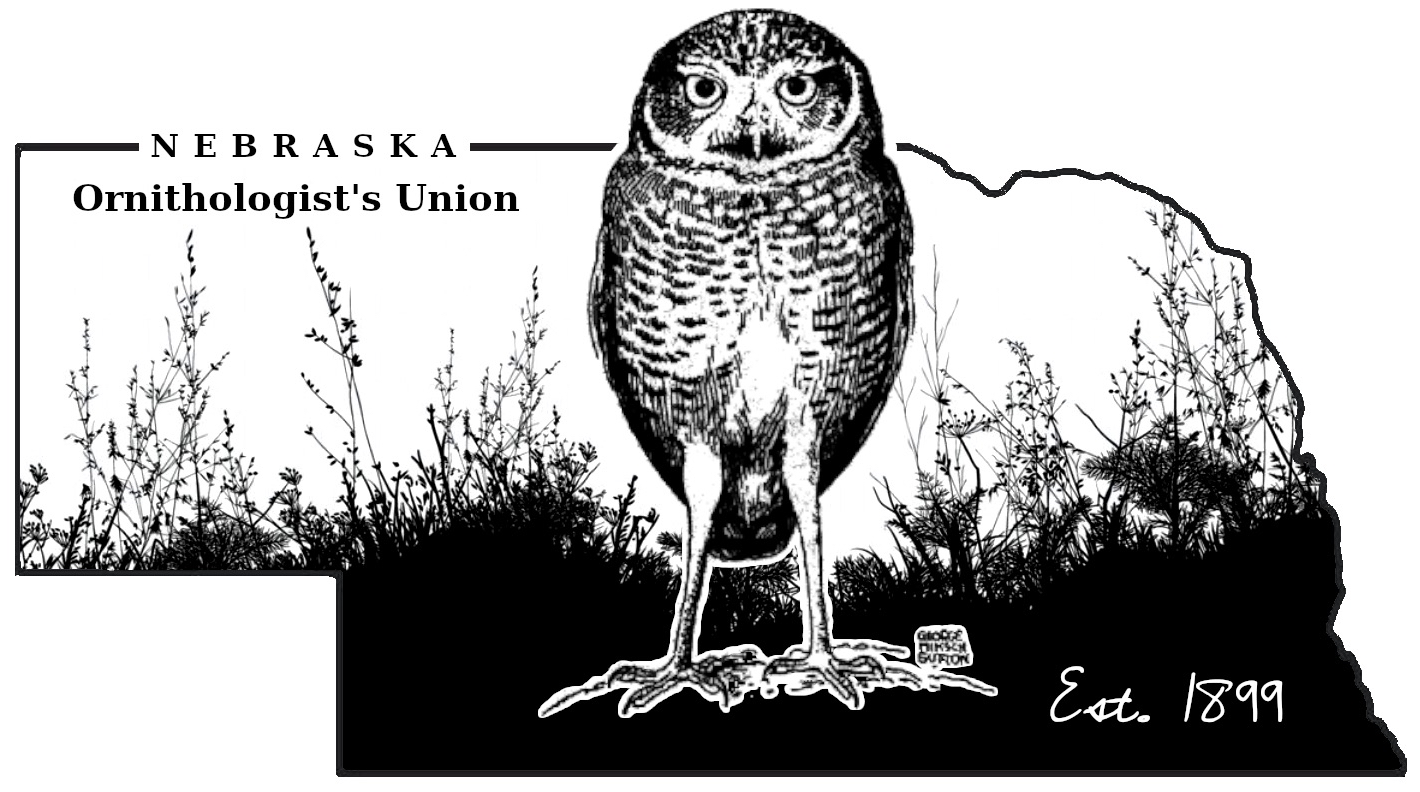
\includegraphics[width=0.42\textwidth,alt={The logo for the Nebraska Ornithologists' Union.}]{./logo/nou_logo.png}
		\\	% this spacer is needed to make the text on the right fit OK
	\end{wrapfigure}
	
	\NewsItem{From the President's Desk}
	\lettrine{F}{ew} would have guessed how spring migration was going to play out for us this year. Well, it was pretty dope. \lipsum[1]
	%\emph{\blindtext}
\end{minipage}
\end{center}
% -----


% Other news (1)
% -----
\vspace{0.5cm}
	\SepRule
\vspace{0.5cm}
\begin{multicols}{3}
	\NewsItem{Monkey eats elephant}
	\NewsAuthor{F. Wenneker}
	\blindtext[2] 
% -----

\vspace{1cm}
% Other news (2)
% -----
\NewsItem{Elephant eats frog}
\NewsAuthor{J. Doe}
	\blindtext[1]
		\begin{center}
			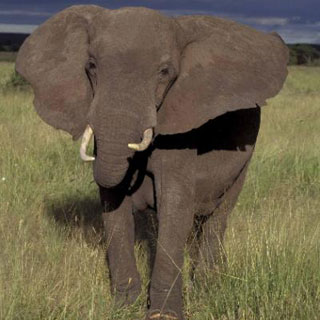
\includegraphics[width=0.8\linewidth,alt={elephant}]{elephant}
		\end{center}
		\blindtext[1]
\end{multicols}

% -----

\end{document} 
